% Chapter 1 of the Thesis Template File
\chapter{INTRODUCTION AND  BACKGROUND}

%This is the opening paragraph to my thesis which explains in general terms the concepts and hypothesis which will be used in my thesis.

%This section will cover the basic and general concepts of my thesis.  This will be a high level approach to the problem and to the proposed solution.  In addition, this section gives a general background to the project

%Chapter 1:  Introduction:
%1) Motivation
%	a) 2-3 sentences on why the felid of Remote sensing important: examples from past and present. [refs]
%	b) 2-3 sentences on what radiometers are (with respect to remote sensing) and examples of how they have been used for remote sensing from the past and more important presently [refs]
%2) Problem
%	a) What aspects of traditional radiometers are limiting their ability to impact society? [refs]
%	b) If these limitations were removed/mitigated, then what additional things could be done with radiometers? [refs or places were radiometers could be useful]
%	c) What high-level approach are you presenting to help address these limitations?  [refs]
%3) Contributions:  2-3 sentences summarizing your contributions (for your thesis you should be able to identify 2 - 3 contributions)
%4) Summary of the organization for the remainder of your thesis

\section{Introduction}
The goal of this thesis is to explore the use of a software defined radio that can function as well as or better than current radiometers.  In addition, we aimed to develop a radiometer that is more flexible than most radiometers and still maintain the accuracy and stability of a traditional radiometers if not exceed these specifications.  A secondary goal was to use off the shelf components that are generally more accessible and often less expensive.  This allows radiometers to be more accessible to a wider scope of researchers in this field.  And finally a tertiary goal was to ensure that the system as a whole is easy to use.  This ties to our secondary goal of making radiometers more accessible to a wider range of researchers and research topics.

This thesis looks to explore the following questions: (1) Can we use an off the shelf SDR along with GNURadio to recreate a radiometer in software that is easy to use and cost effective?  (2) If so, what performance can we get from the system?  (3) What benefits do we gain (if any) from using a SDR from a more traditional radiometer? The results of this research and experimentation are the subject of this thesis.

\subsection{Motivation}
Remote sensing allows us to collect information about the world that is around us.  This information can give us valuable information such as vegetation health, soil moisture, ocean salinity, and astronomy.  

Radiometers are radio receivers that simply listen to and record the amount of power received.  However, the power received is not a coherent signal, instead it is the amount of noise the radiometer sees.  Radiometers, at the basic level, listen to noise that is generated naturally from a source.  These sources can vary and the applications vary as well.  Some examples of radiometer applications have been in evaluating soil moisture content, ocean salinity levels, and celestial objects[\cite{ulaby2014}].

Using radiometers for remote sensing has several advantages as we are able to look beyond certain obstacles that would otherwise be blocked in other remote sensing methods such as photography.  Radiometers have been used in the past for primarily astronomy in scanning for celestial objects that may be hidden from visual telescopes.  More recently radiometers have now been focusing on Earth and helping scientists to better understand the water cycle on Earth by monitoring our ocean salinity and soil moisture.  

\subsection{Problem Statement}
Radiometers have proven to be an excellent tool in remote sensing and have been used in a variety of research applications.  While radiometers have been around for quite some time, the equipment and method of implementing a radiometer has not changed much over the last fifty years.  However, radiometers have not seen much widespread use.  This largely due to the fact that there are very few commercially built radiometers, most radiometers are built to fit a specific purpose or research area.  This is in part due to that different tasks may require changes to the radiometer hardware.  This results in radiometers that are often expensive and require a certain amount of upkeep.  

If though, a radiometer can be built with commercial off the shelf components and also be flexible to adapt to different research or experimental needs, then that type of radiometer will be more desirable and will reduce costs by using available COTS solutions.  

The solution to this problem, as outlined in this thesis, is to create a software defined radiometer that digitizes the incoming radio frequency information as soon as possible and then process this information in software instead of using hardware.  In addition, we will use existing hardware and tools that are commercial available and will be lower in cost or free to the user.  

\subsection{Contributions}
Contributions from the work performed for this thesis include a development of a software defined radiometer that is capable of performing as a radiometer and meets or exceeds the performance of a traditional radiometer.  This includes source code written in the open source software defined radio framework known as GNURadio.  Additional contributions include analysis tools used to analyze data obtained from the software defined radiometer.  Finally contributions were made in using a different technique to mitigate interference that impacts the radiometer readings.  This is accomplished differently from other methods because unlike other radiometers we have both amplitude and frequency information to identify and mitigate this interference.

\subsection{Thesis Organization}
This thesis is organized to first introduce the user to the background and short introduction to both radiometers and to software defined radios.  Next, a more detailed explanation of the theory that allows for a software defined radio to emulate a radiometer in software followed by details on how key components of a radiometer are implemented in software.  We then examine experimental data that was collected to confirm our hypothsis of software defined radiometer and explore advantages a software defined radiometer has over a more traditional radiometer.  Finally we will analyze our results obtained from our experimental data and ensure it meets our expectations for a software defined radiometer.

%----------------------------------------------------------

\subsection{Software Defined Radio Radiometer}

A Software defined radio consist of both hardware and software that allow it to perform the operations of a radio or communication channel.  A software defined radio used for radiometer applications is identical to a software defined radio used for, as an example, a 802.11b radio with one major difference.  Since we need to amplify the signal more than what most communication applications require; we do require more powerful or additional LNAs to boost this signal.  In addition, since the first LNA plays a major role in the overall system noise and this system noise does affect performance of the radiometer, the selection of this LNA is important.  However, all other components are the same components used in other applications.

A software defined radio radiometer behaves analogous to a more traditional radiometer and thus the application is the same as a traditional radiometer.  This includes applications such as radio astronomy that includes applications in Earth Science such as soil moisture and ocean salinity[\cite{Ruf}].  A software defined radio radiometer can also allow for new application development that can expand the remote sensing field.  Since we have moved the majority of the hardware to software this allows us to further shrink the size and weight of the radiometer.  This allows for other radiometer applications such as Unmanned Aerial Vehicles (UAVs) for scanning soil moisture and ocean salinity remotely[\cite{McIntyre}].  

We will now introduce the three major components that make up a software defined radio radiometer.  

%\textbf{N200 SDR}
\subsubsection{N200 Software Defined Radio} 
The key component for a software defined radio radiometer is the software defined radio or SDR that will do most of the work as a radiometer through software.  The equipment selected for researching into this topic was the Ettus Research Group N200 SDR.  The SDR selected utilizes daughter boards as the RF front end to the SDR and up to two daughter boards may be installed into a N200.  This is an important consideration as one of the requirements is to be able to look at both the V-Pol and the H-Pol signal coming from the antenna.  By having a dual receiver SDR it is possible to correlate the signal and other signal analysis can also be done.  Another important reason the N200 is selected was due to its ability to handle up to 50 MHz of bandwidth to the computer and up to 25 MHz of RF bandwidth per daughter-board plugged in to the SDR.  This means that it is possible to have two receive cards that can stream up to 25 MHz bandwidth each.  

The N200 utilizes a flexible architecture for a variety of RF interface systems based on the frequency range desired and if receive and/or transmission is needed.  These daughter boards directly receive the RF signal and then outputs the analog I and Q signals that are then sampled by the N200 A/D converter for reception or receives the I and Q values from the N200 D/A converter for transmission. 

{\begin{figure}[h!tb] 
\centering
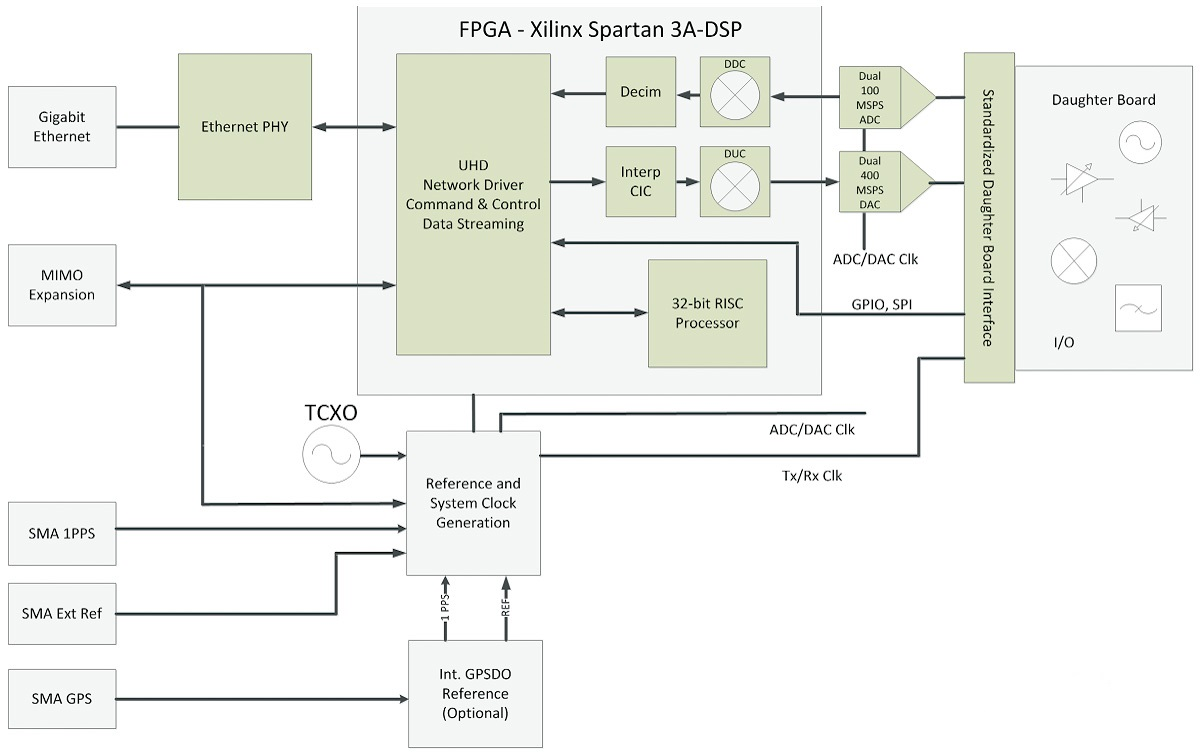
\includegraphics[width=14cm]{Images/n200_block_edited}
\isucaption{A block diagram of the Ettus N200 SDR}
\label{N200_block}
\end{figure}
}

The daughter board selected is the DBSRX2 card as this card is receive only and operates between 800 MHz and 2.4 GHz.  The DBSRX2 also has built in amplification that is adjustable through software.

\subsubsection{GNURadio Software}

For the software portion of the radio, we settled to use GNURadio, an open source software package that is well supported by the community and by the Ettus Research Group and the N200 SDR.  GNURadio also comes with what is known as GNURadio Companion or GRC.  This program provides us with a GUI interface and allows for the drag and drop of blocks that represent certain functions that can be used with the SDR.  GNURadio and GRC use Python as its main scripting language and GNURadio uses C++ code for directly accessing the hardware.  The hardware interface for the N200 is provided by Ettus through drivers that allow GNURadio to talk to the hardware.  Like GNURadio, these drivers are also available to all platforms.  Ettus has released these drivers to the open source community and continues to support the hardware drivers and GNURadio integration.

GNURadio operates on multiple platforms including Windows, Mac OS X, and Linux.  Linux is by far the most popular platform to work on and most of this thesis research was completed within the Linux environment.  Testing is also done though with a MacBook Pro running OS X 10.9.  The OS X implementation is well supported and is installed through MacPorts.  While windows is technically supported, it is often difficult to install and many of the libraries required are not 64-bit.  For these reasons windows was not used for executing GNURadio, but was used for some of the data analysis using Python.

Through GNURadio, we can now write code that will take the data given to us from the SDR and manipulate the signal as we need to mimic a radiometer.  The power detection, filtering and recording of this data is all done through GNURadio.  This also means that we are shifting more of the computational power done on the signal from the FPGA to a computer running GNURadio.  There are ways to change this behavior and upload code directly to the FPGA.  However, for this thesis it was easier to debug and work with GNURadio by keeping the processing on the desktop computer.  It does however mean that the host computer must be powerful enough to handle the signal and specifically the large bandwidth that we wish to send to it.  

\subsection{RF Front End}
The RF front end plays a critical role in the radiometer as the LNAs used in the front end has a large impact on the system noise generated by the radiometer itself.  A traditional radiometer utilizes both amplification through the LNAs and also includes filtering to the desired bandwidth.  A SDR radiometer does not require the filters as we are able to create these in software, however the amplification stages need to remain.  

{\begin{figure}[h!tb] 
\centering
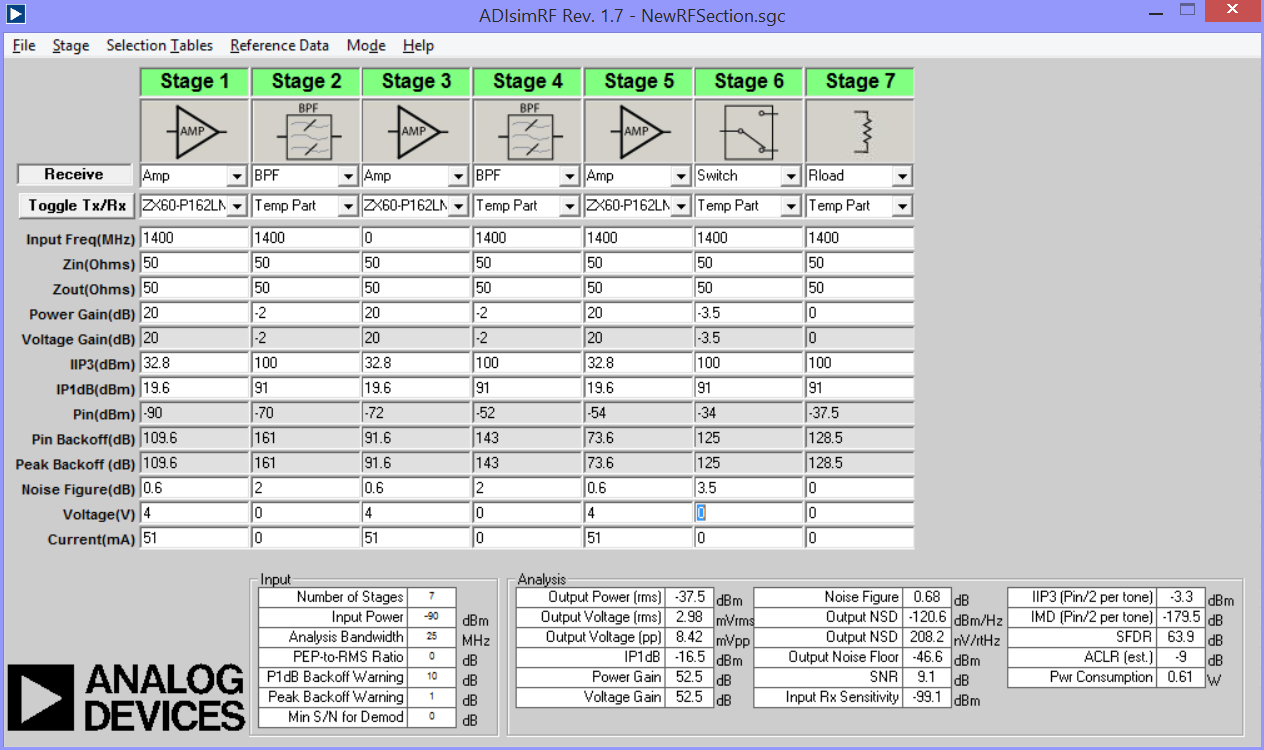
\includegraphics[width=0.8\linewidth]{Images/RF_Front_end.png}
\isucaption{The ADISIMRF program used to verify the design of the RF Front End}
\label{ISU_Rad}
\end{figure}
}
A typical RF front end uses a 3 stage Low Noise Amplifier (LNA) to amplifier the noise while keeping the noise contributed to the system as low as possible.  As with any radiometer, the first LNA is the most critical as it contributes the most to the overall system noise temperature.  For this reason a LNA that did not have a large gain but had a low noise figure is chosen. The second and third LNA has higher gain values at the cost of a higher noise figure, although not by much.  However, since they are further down the chain, they do not contribute as much to the total system noise.  The reason for this is further explained in chapter 3. 